\documentclass[journal]{IEEEtran}
\usepackage[portuguese]{babel}
\usepackage[portuguese]{babel}
\usepackage[utf8]{inputenc}
\usepackage[T1]{fontenc}
\ifCLASSINFOpdf
\else
\fi
\hyphenation{op-tical net-works semi-conduc-tor}

\usepackage{caption}
\usepackage{graphicx}

\begin{document}
\title{Extensão do GCC Através de Plugin}

\author{Guilherme Zamberlam Pomini}
\markboth{Journal of IEEE Latin American Transactions,~Vol.~4, No.~1, Janeiro~2020}%
{Shell \MakeLowercase{\textit{et al.}}: Bare Demo of IEEEtran.cls for IEEE Journals}
\maketitle
\begin{abstract}
Um compilador para a computação é um programa cujo objetivo é traduzir um objeto de uma linguagem de origem para uma linguagem de destino, é através de um compilador que o programador consegue gerar programas executáveis a partir de diversas linguagens de programação. Uma das tarefas do compilador é realizar uma análise do código-fonte para tomar decisões posteriormente. Embora os compiladores já possuam um padrão de análise, esse comportamento pode ser estendido de acordo com a necessidade com plugins. Este artigo traz a implementação de um plugin para o compilador GCC com o intuito de gerar uma análise detalhada de características presentes no código-fonte de um programa. Com a implementação do plugin foi possível obter dados importantes sobre os programas, como número de blocos básicos, quantidade de instruções, número de constantes, entre outras informações.
\end{abstract}
\begin{IEEEkeywords}
Compiladores, GCC, Plugin
\end{IEEEkeywords}
\IEEEpeerreviewmaketitle

\section{Introdução}

\IEEEPARstart{D}{entro} do escopo da computação programadores podem desenvolver seus programas nas mais variadas linguagens, variando de acordo com a necessidade do programador. No entanto, apesar da possibilidade de representar um programa em diversas linguagens, a máquina que vai executar o programa de fato espera uma entrada em um formato que ela saiba ler, e posteriormente executar.

Como forma de auxiliar o programador na comunicação com o computador, nasceram os compiladores. Um compilador é um programa cujo objetivo é fazer uma transformação de uma linguagem fonte para uma linguagem alvo (não necessariamente a linguagem final para o computador) interpretando e ajustando o código de acordo com a necessidade \cite{livro}.

O uso mais comum de um compilador é a geração de um executável a partir de um código-fonte. Contudo essa não é a única função de um compilador, mesmo sem gerar um arquivo final ainda é possível tirar proveito das funcionalidades de um compilador. Uma possibilidade comumente utilizada é a análise do código-fonte, sendo frequentemente feita por plugins. A criação de um plugin permite a adição de novas funcionalides ao compilador sem a necessidade de recriar o compilador \cite{GCC-DOCS}, sendo uma poderosa ferramenta para um desenvolvedor que pode criar plugins conforme a sua necessidade.

Este trabalho visa a extensão das funcionalides do compilador GCC \cite{GCC} através da implementação de um plugin. O plugin planejado irá realizar uma análise do código-fonte do programa alvo para extrair características pré-definidas.

\section{Desenvolvimento}

A construção de um plugin para o GCC trabalha em cima da notação de código intermediário GIMPLE, padrão do GCC. Para realizar de fato a análise do código-fonte em formato GIMPLE foi utilizada a própria API do GCC que fornece métodos de acesso para as diversas estruturas intermediárias geradas, conseguindo assim acessar todo o código gerado pelo GCC \cite{gcc2}.

Dito isso, o presente trabalho focou na implementação de um plugin que realize a extração de 56 características estáticas de código que visam auxiliar na decisão de otimizações de código realizadas pelo compilador \cite{features}. Algumas características que visam ser extraídas são: quantidade de blocos básicos, quantidade de instruções, quantidade de arestas no grafo de fluxo, quantidade de nós phi, quantidade de constantes, entre outras.


\section{Metodologia e Resultados}

Para realizar os testes com o plugin implementado foram utilizados 10 programas de diferentes benchmarks. Como forma de testar o funcionamento do plugin foram escolhidas algumas características para avaliação entre os programas.

\subsection{Metodologia}

\begin{itemize}
    \item \textbf{Ambiente:} Linux Mint 19, Processador I5 7ª Geração, 8GB de Memória RAM
    \item \textbf{Versão GCC:} 9.2.0
    \item \textbf{Linguagem do Plugin:} C++
    \item \textbf{Progamas Utilizados:} CrystalMK (Benchmark ASC\_Sequoia, um micro kernel), fannkuch (Benchmark BenchmarkGame), uuencode (Benchmark BitBench), almabench (Benchmark CoyoteBench), fldry (Benchmark Dhrystone), flops (Benchmark Misc, estimativas com ponto flutante), dc (Benchmark NPB-Serial), matrix (Benchmark Shootout), sim (Benchmark sim, algoritmo de programação dinâmica) e bmm (Benchmark VersaBench, realiza a soma de uma multiplicação de matrizes)
    \item \textbf{Características Analisadas:} Quantidade de Blocos Básicos, Quantidade de Chamadas Diretas e Quantidade de Saltos Condicionais.
    \item \textbf{Experimentos:} Como a análise é realizada em diretamente no código fonte, cada programa foi analisado uma única vez, não necessitando repetições. Como o plugin gera dados tanto para cada função do arquivo como para a soma de todas as funções, nos experimentos foram utilizados somente os valores das funções somadas.
\end{itemize}

\subsection{Resultados}

A partir das características extraídas de cada programa, foram feitos gráficos para exemplificar uma breve análise das caracteríticas e validar a implementação do plugin.

Como forma de normalizar os resultados devido a diferença de tamanho entre os programas, as características de Quantidade de Chamadas Diretas, e Quantidade de Saltos Condicionais aqui estão em proporção à Quantidade de Blocos Básicos, como mostra a Figura ~\ref{graph}.

\begin{figure}[h]
\centering
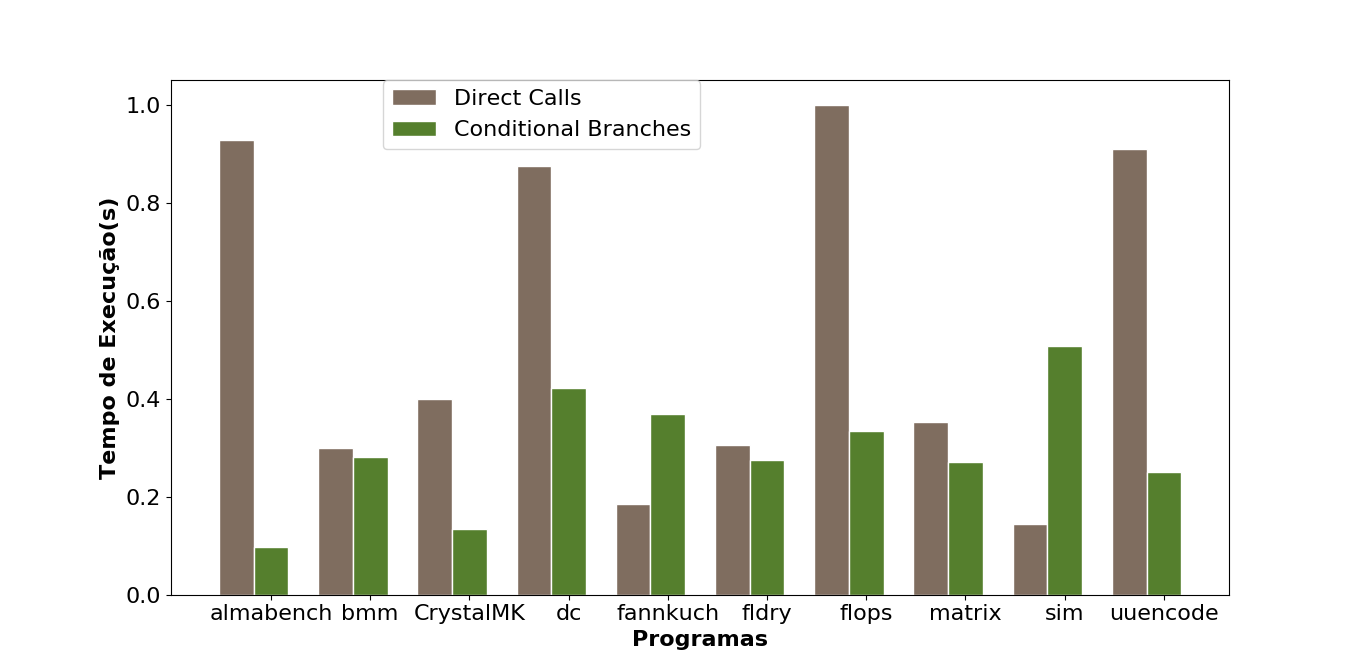
\includegraphics[width=3.5in]{graph.png}
\captionsetup{justification=centering}
\caption{Quantidade de Chamadas Diretas e Quantidade de Saltos Condicionais}
\label{graph}
\end{figure}

Analisando o gráfico da Figura ~\ref{graph} é possível notar que em geral a quantidade de chamadas diretas é superior a quantidade de saltos condicionais, sendo exceções somente os programas Fannkuch e Sim. Com uma informação dessas em um cenário onde só poderia escolher 1 tipo de otimização para todos os programas, escolher otimizar as chamadas diretas resultaria em um desempenho melhor em 80\% dos programas.

Com isso foi possível validar o funcionamento do plugin, bem como a importância da análise das características extraídas pelo mesmo.

\section{Conclusão}

Os compiladores são programas fundamentais para a ciência da computação como um todo, abstraindo inúmeros procedimentos que realizam a comunicação de fato entre um programador e o computador. Um importante procedimento que o compilador realiza é a análise do código-fonte, procedimento este que pode ser estendido através de plugins.

Este trabalho visou a implementação de um plugin para o compilador GCC com o objetivo de extrair informações sobre o código-fonte de um programa. Com a execução do plugin implementado foi possível realizar uma análise de código-fonte de 10 diferentes programas, extraindo informações como quantidade de blocos básicos, quantidade de chamadas diretas, quantidade de saltos condicionais, entre outras.

Através das informações coletadas foi possível por exemplo escolher otimizações de código que mais impactariam positivamente o resultado final da maioria dos programas. No caso analisado, foi encontrada uma possível rota de otimização que seria a melhor para 80\% dos programas analisados.

Ao final do trabalho o plugin implementado serviu ao seu propósito de maneira satisfatória, extraindo informações como era desejado.

\begin{thebibliography}{1}

\bibitem{livro}
A.~V. Aho, et al. , \emph{Compilers, Principles, Techniques and Tools}, 2rd~ed.\hskip 1em plus
  0.5em minus 0.4em\relax  2007.
  
\bibitem{gcc2}
CALLANAN, Sean; DEAN, Daniel J.; ZADOK, Erez. Extending GCC with modular GIMPLE optimizations. In: Proceedings of the 2007 GCC Developers’ Summit. 2007. p. 31-37.

\bibitem{features}
Mircea Namolaru, Albert Cohen, Grigori Fursin, Ayal Zaks, Ari Freund: Practical aggregation of semantical program properties for machine learning based optimization. CASES 2010: 197-206
  
\bibitem{GCC}
 Using the GNU Compiler Collection (GCC). [Online]. Disponível em: https://gcc.gnu.org/onlinedocs/gcc/index.html. [Acesso em 29 dez 2019].
 
\bibitem{GCC-DOCS}
 GCC Documentation - Plugins. [Online]. Disponível em: https://gcc.gnu.org/onlinedocs/gccint/Plugins.html. [Acesso em 29 dez 2019]
  
\end{thebibliography}

\bibliography{bib}

\begin{IEEEbiography}
[{
\includegraphics[width=1in,height=1.25in,clip,keepaspectratio]{foto.jpg}}]{Guilherme Zamberlam Pomini}
Graduando do quarto ano em Ciência da Computação na Universidade Estadual de Maringá, UEM
\end{IEEEbiography}
\end{document}


